\documentclass[titlepage]{report}

\UseRawInputEncoding

\usepackage[toc,page]{appendix}
\usepackage[toc,section=section]{glossaries}
\usepackage{imakeidx}
\usepackage{biblatex}
\usepackage{graphicx}
\usepackage{float}
\usepackage{listings}
\usepackage{selinput}
\usepackage{changepage}

\lstset
{
    language=Python,
    basicstyle=\footnotesize,
    numbers=left,
    stepnumber=1,
    showstringspaces=false,
    tabsize=1,
    breaklines=true,
    breakatwhitespace=false,
}

\lstset
{
    language=bash,
    basicstyle=\footnotesize,
    numbers=left,
    stepnumber=1,
    showstringspaces=false,
    tabsize=1,
    breaklines=true,
    breakatwhitespace=false,
}

\lstset
{
    language=C,
    basicstyle=\footnotesize,
    numbers=left,
    stepnumber=1,
    showstringspaces=false,
    tabsize=1,
    breaklines=true,
    breakatwhitespace=false,
}

\makeglossaries{}
\loadglsentries{entries}

\indexsetup{level=\section}
\makeindex
\addbibresource{bib.bib}

\title{blockchain\_message: A Peer-to-Peer Content-Sharing Service Built on the Ethereum Blockchain\\\large{System Documentation}}
\author{Sean T. Batzel\\Dr.\ Bishop}
\date{\today\endgraf\bigskip Submitted in partial fulfillment of the requirements of CMPS/IT 490 --- Computer Projects}

\begin{document}
\maketitle

\tableofcontents

\nocite{*}

\begin{abstract}
The Ethereum\index{Ethereum} network has attracted a considerable volume of attention in recent months for its native currency, Ether.\cite{ethereum} During the cryptocurrency\index{cryptocurrency} bubble beginning in early 2017 and apparently ending nearly a year later the value of Ether\index{Ether} skyrocketed from just a few dollars to over a thousand dollars. It attracted a staggering number of investors hoping to make a fortune speculating on the value of Ether\index{Ether}, Bitcoin\index{Bitcoin}, and other currencies. Now that the prices have leveled off, the noise has died down somewhat, but is Ethereum's\index{Ethereum} usefulness over? Ethereum\index{Ethereum} itself was never intended as an investment vehicle. Ether was originally conceived of as a way to handle time-sharing on a distributed computing platform. The Ethereum Virtual Machine\index{Ethereum Virtual Machine} itself was designed as a sort of "world computer" which can be used to distribute and run theoretically any program that can be conceived of. People deploying their distributed applications to the EVM\index{Ethereum Virtual Machine} or requesting processing time from one of those applications pay a \gls{gas}\index{gas} fee which sets an upper limit on the amount of time an operation can take on the machine.\cite{yellowpaper} The goal of this project is to provide a client/server-analog which uses the Ethereum virtual machine\index{Ethereum Virtual Machine} and \gls{blockchain}\index{blockchain} as the middleware and backend of an email-type service.
\end{abstract}

\chapter{Overview}

Since email, instant messaging, and SMS are all commonplace in technology this project may seem to simply reinvent the wheel. These services, though all practical and convenient, tend to be held by a particular group of companies or entities. Content sent between two participants in a conversation are not sent directly from person to person; there must be some intermediary to handle delivery. This project will take advantage of the transaction structure of the blockchain\index{blockchain} and use Ethereum\index{Ethereum} as the delivery and storage system. By committing messages to Ethereum, the ownership and control of the content a party is sending is maintained by the holder of the private keys for the origination of transactions and for the decryption of messages sent to the chain.\\

\begin{figure}[h]
    \centering
    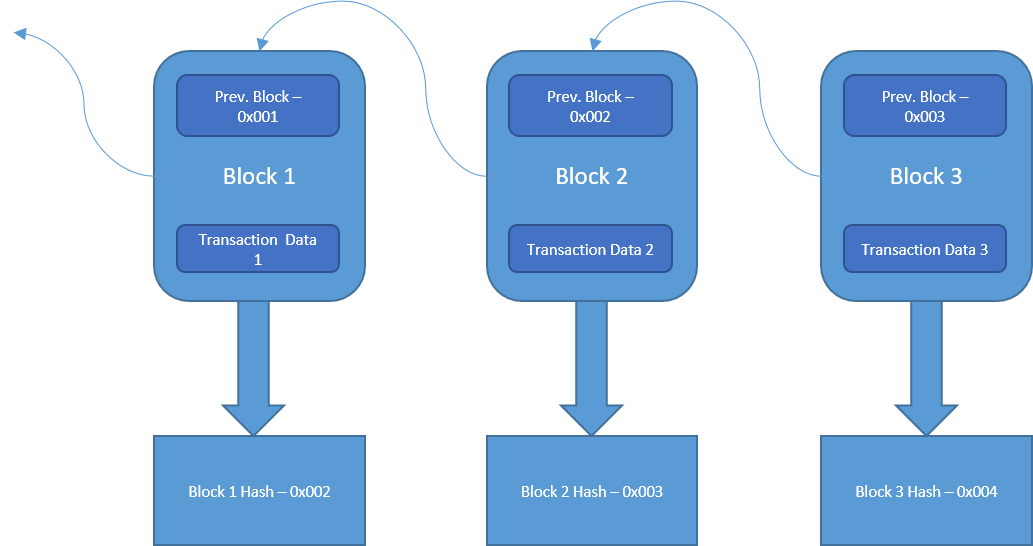
\includegraphics[width=0.5\textwidth]{blockchain}
    \caption{A closer diagram of a general-purpose blockchain. Blocks are connected from one to the next with the capability of adding data payloads to each transaction - in this case, unicode-encoded messages.}
\end{figure}

Consider two conversation partners, Alice and Bob. Bob sends a text message to Alice, which is sent from his device to his carrier. It is relayed through cell towers and data centers, stopping along the way in some unknown number of locations and being saved. Finally it will eventually be delivered, not by the device itself but by the combination of cell carriers, to Alice. There is no promise of security, privacy, or control over the data being sent between endpoints. A message delivery service built on Ethereum\index{Ethereum} would, by nature, circumvent these concerns. Everything occurring on the Ethereum virtual machine\index{Ethereum Virtual Machine} is committed to the blockchain\index{blockchain}. This occurs by distributing every \gls{transaction}\index{transaction} to every computer running a copy of the core Ethereum\index{Ethereum} software. Because every \gls{node} has a copy of that action, it is by definition decentralized. Each transaction is also associated with a pair of public keys (called addresses in cryptocurrency\index{cryptocurrency}), which allows them to prove their origin and destination. As the chain is processed by a number of computers (called miners) tasked with validating and verifying the integrity of the chain\footnote{This is done by using a high-difficulty hashing algorithm to verify that each transaction is a valid extension of the former state of the blockchain\index{blockchain}.}, each \gls{miner}\index{miner} checks to make sure that every one of these transactions, and the metadata associated with them, is completely correct in relation to the rest of the \gls{blockchain}. This allows us to be absolutely certain that every message that this application sends or receives is immutably and provably present.\cite{blockchain}\\

\begin{figure}[h]
    \centering
    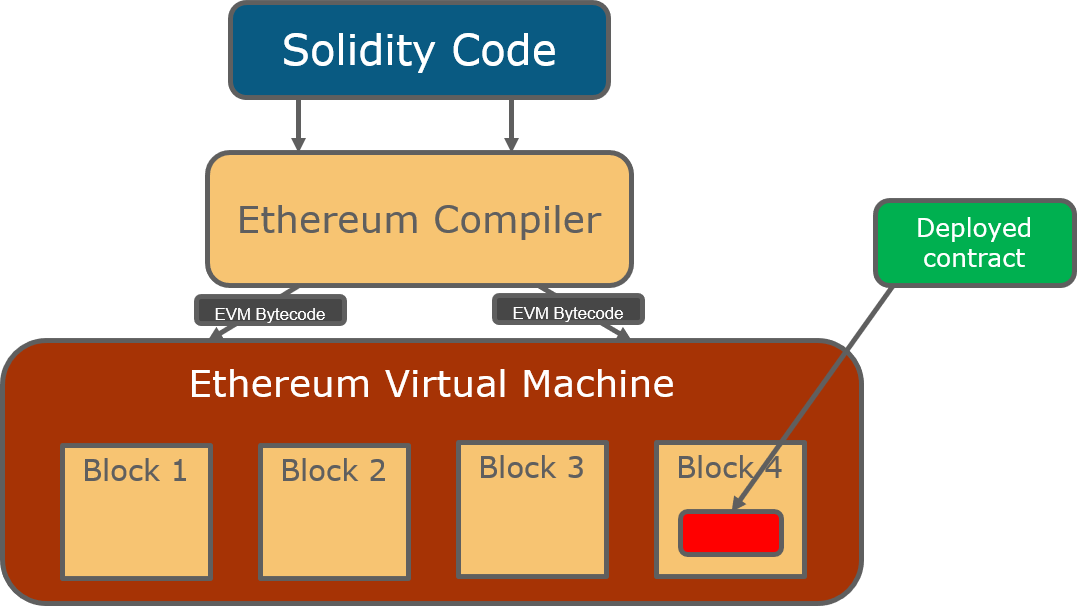
\includegraphics[width=0.5\textwidth]{ethereum}
    \caption{The Ethereum virtual machine functions by distributing bytecode to a number of connected computers, which then execute the given bytecode.}
\end{figure}

On the technical end, this project will ostensibly consist of a database module which will allow us to store content client-side, a cryptographical module using Python's RSA\index{RSA} module, and a blockchain\index{blockchain} module which will allow us to communciate directly with a local version of Ethereum through web3. These functions will all be internal, with a set of functions exposed to the end-user for interacting with the project as a library.\\

I intend for this project to be a proof-of-concept library written in Python\index{Python}. It will require a Python\index{Python} version greater than 3.6, as well as the \gls{web3}\index{web3} implementation for Python\index{Python}.\cite{web3-py} For testing purposes it will also require a \gls{test RPC}\index{test RPC} installed locally in order to test and debug the \gls{smart contract}s\index{smart contract} associated with the application. This smart contract will require a Solidity compiler to be installed in order to produce the compiled bytecode for the contract. In order to maintain the privacy of the messages sent to the blockchain, the library will make direct use of RSA\index{RSA} keypairs to send encrypted messages between users. The test RPC\index{test RPC} I plan on using (Ganache\index{ganache}) will require that the latest version of Node.js\index{Node} installed on the local system. The process of deploying the contract\index{smart contract} and interacting with it will be handled entirely by Python\index{Python} scripts, and in order to deploy the contract\index{smart contract} to the Ethereum\index{Ethereum} \gls{mainnet}\index{mainnet} an RPC pointed at the Ethereum Foundation's official blockchain will be necessary. All of these may be easily installed on most operating systems.\\

The core functionality of the CLI client has been implemented fully. The database\index{database} and cryptographical\index{cryptographical} modules will be comparatively simple to implement. In terms of goals I would like to reach but which may be more challenging, the current project uses a full local Ethereum\index{Ethereum} node to communicate with the network. The storage requirement for a full node is O(n) where n is the number of transactions\index{transaction} in the blockchain\index{blockchain}. This is impractical for devices with smaller available storage, so the implementation of a \gls{light client}\index{light client} (with storage requirement O(log(n))) integrated into the system would simplify setup and reduce resource usage considerably. The aim for the Ethereum-based portion of this project is to implement an efficient enough smart contract to optimize the gas usage of the system and thereby retain reasonable transaction fees for users of the service.

\chapter{blockchain\_message}
\section{Introduction}
A major point of concern in computing in general recently has been privacy. What are companies doing with our data to leverage us as assets? If I send an email or a text message, or even make a phone call, who is privy to what's said in those communications? Can we conclusively trust the services we use? blockchain\_message is a platform which utilizes the new and growing blockchain model through Ethereum, along with time-tested encryption processes to allow for the transmission of information securely and directly, using a decentralized network to process the messages rather than a single entity. Using Ethereum, the system is designed to make messages as difficult to intercept, modify, delete, or otherwise disrupt as possible, working to make your communications as secure as they can be.

\pagebreak
\section{System Model}
\begin{figure}[H]
    \centering
    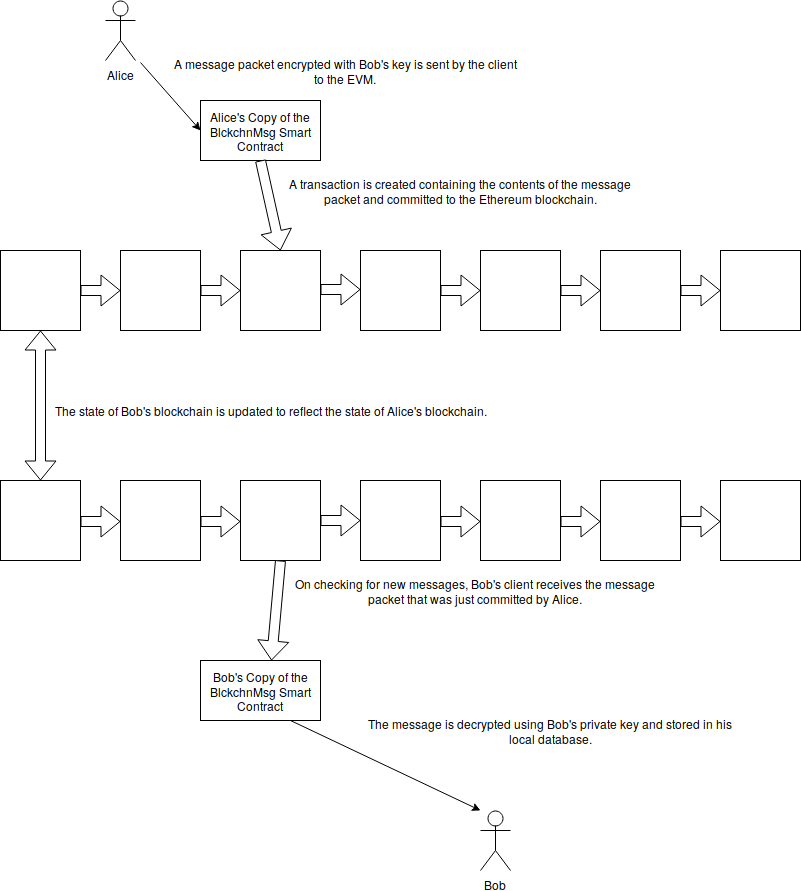
\includegraphics[width=1.3\textwidth]{diagram}
    \caption{A high-level overview of blockchain\_message's functionality.}
\end{figure}
\pagebreak

\section{Functional Requirements}
\subsection{General Features Overview}
The base functionality of the application is a simple instant messaging system where messages are exchanged directly through \gls{Ethereum}\index{Ethereum} and not through a central server. Messages are encrypted and sent to a program running on the Ethereum computer, which records them in a permament and unchangeable chain to be downloaded and decrypted by the intended recipient. Ideally, users of this platform would be able to create an account for a single device that would remain completely secure for every communication sent from it.

\subsection{Security and Privacy}
The major benefit to this system being built on Ethereum\index{Ethereum} is that every message sent is recorded permanently in a transaction\index{transaction} on the blockchain\index{blockchain} in a manner that, because of Ethereum's architecture, cannot be changed. Because fairly strong RSA keypairs are used for encryption/decryption purposes, the messages are committed in such a way that it becomes prohibitively challenging to hijack them, whether to read them or to modify them. If used correctly, the system will create a new keypair for every device (assuming that the same identity is not used on multiple devices), reducing the risk that decryption keys may be stolen. Data is encrypted and committed to the blockchain on the local machine, reducing the risk that unencrypted data may be intercepted during communication. This also removes the privacy concerns for services using the standard server/client architecture, since the data is stored on every node running Ethereum there are no concerns for losing access to one's personal data.

\section{User Interface Specification}
The UI will have three levels during development, starting with a command-line interface, with a median goal being an HTML5-based graphical interface and the ultimate goal being a native Android application.

\subsection{Command-Line Interface}
The CLI will accept a few simple commands for interacting with the blockchain\_message system. On running the program, you will be met by a login screen to prompt for a username, an email address, and a password. These three elements will be used to identify you to the network while exchanging messages.
The interface commands are as follows:

{\raggedright{}
    \texttt{balance} - Check the Ethereum account's balance. This volume of Ether is used to fuel the transfer of messages.\\
    \texttt{check} - See if any new messages have been received.\\
    \texttt{read} - Read all of the messages we've already downloaded.\\
    \texttt{write} - Compose, encrypt, and send a new message. This will prompt for a username to send to, followed by message text. All other steps are handled automatically.\\
    \texttt{contacts} - List the user's current contacts.\\
    \texttt{new-contact} - Create a new contact object. This will prompt for a username and will find the target's address automatically. A public key for the given username must be found in the \texttt{client/.keys/} directory.\\
    \texttt{help} - Display this command list as a help dialog in the context of the running program.\\
    \texttt{exit} - \textit{Always} use this to end the program. It's responsible for ensuring the application's internal state saves correctly.\\
}

\subsection{HTML5 Interface}
As a medium-term stretch goal, I plan on implementing a simple graphical interface running locally for end users who are less comfortable with CLI operations. The HTML5-based interface will expose all of the same functionality as the command-line interface.

\subsection{Android Application}
My extreme-term stretch goal is to develop and Android application that leverages the light client specification to run the entire application locally to an Android device. The app itself will consist of a standard navigation menu with a screen for contact management (add/delete/edit/detail functions will also be exposed), a screen for message management (with the standard functionality expected from a messaging client), and a screen for profile management which will allow sharing profile information and public encryption keys.

\section{Non-functional Requirements}
\subsection{Software Requirements}
The first version of the blockchain\_message command-line interface is designed to run on Ubuntu Linux\index{Linux}, but with tweaking can be made to run on any system with Python installed. The installation script can be easily modified for installation on any Linux distribution.

The system requires that an Ethereum\index{Ethereum} \gls{node}\index{node} be accessible, which can be either set up on the local machine through Parity or Geth or exposed through a service such as Infura.io. A long-term goal is to leverage the light client specification to create a version that requires less heavy-duty hardware, allowing smaller computers and smartphones to run the system.

The latest version of Python (at the time of writing, 3.6.6 is installed locally) is required, as well a list of Python packages that are installed by the \texttt{install} script. These requirements are laid out in Table 1.

\begin{table}
    \begin{center}
        \begin{tabular}{| l | p{5cm} |}
            alabaster\\
            attrdict\\
            Babel\\
            base58\\
            certifi\\
            chardet\\
            cytoolz\\
            docutils\\
            eth-abi\\
            eth-account\\
            eth-hash\\
            eth-keyfile\\
            eth-keys\\
            eth-rlp\\
            eth-typing\\
            eth-utils\\
            hexbytes\\
            idna\\
            imagesize\\
            ipfsapi\\
            Jinja2\\
            lru-dict\\
            MarkupSafe\\
            packaging\\
            parsimonious\\
            py-solc\\
            pyasn1\\
            pycryptodome\\
            Pygments\\
            pyparsing\\
            pytz\\
            requests\\
            rlp\\
            rsa\\
            semantic-version\\
            six\\
            snowballstemmer\\
            Sphinx\\
            sphinxcontrib-websupport\\
            toolz\\
            urllib3\\
            web3\\
            websockets
        \end{tabular}
        \caption{Python environment package requirements.}
    \end{center}
\end{table}

\subsection{Hardware Requirements}
\subsubsection{If Using a Local Ethereum Node}
If you're using a node\index{node} set up on another system, ignore this paragraph. If Parity, Geth, or a similar Ethereum node is running on the local machine, blockchain\_message requires available resources for both the appliation itself and the Ethereum node. The entire Ethereum blockchain\index{blockchain} will require approximately 300 gigabytes of disk space and 4 gigabyte of available memory. Usually, it's preferable to have 2 CPU cores for blockchain\index{blockchain} operations

\subsubsection{blockchain\_message Requirements}
The blockchain\_message process itself will require a safe minimum of 250 megabytes of available disk space and 50 megabytes of available memory.

\subsection{Product Standards}
\subsubsection{Data Representation}
The data objects that blockchain\_message is concerned with will be stored in memory as a series of interlocking Python objects stored in an overarcing \texttt{Database} object, using the \texttt{shelve} module for object persistence. The \texttt{Database} object consists of a \texttt{Message} list and a \texttt{Contact} list.

a \texttt{Contact} consists of an identifying integer referred to as the ``user address'', a unique username, an email address, and an RSA public key.

A \texttt{Message} consists of a unique identifying number, the user address of the sender, the user address of the recipient, the text of the message, and the RSA signature of the encrypted message text.

\subsubsection{User Manual}
\subsubsection{Programming Manual}
The documentation will be generated from standard Python docstrings by the Sphinx utility for Python.

\subsection{Process Standards}
\subsubsection{Code Quality/Convention}
The codebase for this project should adhere strictly to PEP-008 stylistic guidelines and to idiomatic Python. It will be strictly held to standard Pythonic convention with each individual portion of the functionality separated into its own class or function.

\subsubsection{Comment Quality/Convention}
Inline comments should be avoided unless absolutely necessary, since special care should be taken to ensure that code is idiomatic, readable, and clear.

\section{System Evolution}
\subsection{Assumptions}
A key set of assumptions must be made and proven in order for blockchain\_message to function as expected.
\begin{itemize}
    \item The Ethereum blockchain may be used to store arbitrary data in a structured format.
    \item RSA Encryption allows for identity verification through key signing.
    \item Ethereum transactions are conclusively 
\end{itemize}

\subsection{RSA Web-of-Trust}
RSA's keysigning utilities will eventually be leveraged so that a user of the system can add a new contact and provably verify that that person is who they claim to be.

\subsection{Cross-Platform CLI}
At the time of writing, the CLI is explicitly written for easy installation and running under an Ubuntu Linux environment. Eventually, the existing installation scripts will be redesigned to install dependencies in a distribution-agnostic manner, and scripts (.ps1 or .bat) will be written to allow for simpler running on Windows.

\subsection{HTML5 Interface}
The HTML5 interface will run on a local server with a web interface exposed on a specified port and using the blockchain\_message library as the bulk of the application logic.

\subsection{Android Application}
As a major stretch goal, this project will include an eventual Android application that leverages Ethereum's Light Client Specification to run the entire environment locally on a smartphone. Rather than loading the entire blockchain, a Light Client reads only transactions directly pertaining to its own loaded accounts, therefore reducing the amount of disk space needed and allowing the necessary transactions to be sent to the chain without relying on an external system to host the Ethereum node.

\chapter{Justification and Feasibility}
\section{Justification}
The goal in writing this system is to present a substantial proof for the general-purpose utility of the Ethereum\index{Ethereum} \gls{smart contract}\index{smart contract} system when leveraged by a dedicated client. It also attempts to prove a reasonable feasibility for the possibility of fully-decentralized\index{decentralized} correspondence.

The concept of a \gls{blockchain}\index{blockchain} itself has gained serious traction recently, with a number of concerns online that Bitcoin\index{Bitcoin}, Ethereum\index{Ethereum} and other cryptocurrency platforms are ``dead''\footnote{A quick look at Google results for ``Ethereum\index{Ethereum} dead'' returns a number of results, mostly market analyses claiming that the investment vehicle has become irrelevant.} since the price of the connected cryptocurrencies has dropped so rapidly in recent months. Though Ethereum\index{Ethereum} has gained a considerable following for its internal commodity Ether\index{Ether} (ETH), the original purpose of the network was as a ``world computer'' on which programs (called ``smart contracts''\index{smart contract}) could be run in a manner similar to the time-sharing done on early computers.

The decentralization\index{decentralization} of the Ethereum\index{Ethereum} environment also presents a driving factor for the importance of this system. The vast majority of applications intended for sending content or, more generally, information between two endpoints rely heavily on the existence of a centralized server infrastructure where said information resides until such time as the body owning the server decides it should be purged. While it exists on the server, it can often be considered as transitively belonging to the organization to which the server belongs.\footnote{An End User License Agreement for most services will often outline the data rights of both the licensor and the licensee. Many of these may include language to allow use of data for various purposes. Refer to such articles as Singer, 2018.\cite{singer}} Worrying about such things may bear the appearance of fear-mongering or needless distrust, but there are genuine concerns for the privacy and safety of personal data. This service provides a simple and relevant example for how Ethereum\index{Ethereum} may be used to contribute to the improvement of straightforward data safety based on the general principles of how the blockchain\index{blockchain} paradigm functions.

We can provide strong evidence for the cryptographical security of the blockchain\index{blockchain} paradigm as set forth in the original whitepaper for Bitcoin\index{Bitcoin}.\cite{nakamoto} Data embedded in the blockchain\index{blockchain} is proposed by a single \textit{\gls{node}}\index{node}. This node contains a full copy of the entire ledger for the ecosystem (such as Bitcoin\index{Bitcoin} or Ethereum\index{Ethereum}) which is distributed to all computers running nodes\index{node} along with a cryptographic justification for the adoption of that as the reality of the blockchain\index{blockchain}. Under the current consensus model, these justifications are exhaustively verified and proven by \textit{\glspl{miner}}\index{miner} which continuously prove the justifications for each new block of transactions introduced to the blockchain\index{blockchain}. This becomes relevant to a content-sharing framework in that every message committed to the network is etched permanently in the collective memory of the "world computer". As long as Ethereum\index{Ethereum} functions as set forth in the yellow paper\cite{yellowpaper}, these messages are unable to be removed or changed.

In its current conception, blockchain\_message uses RSA public-key encryption in order to supplement the data and identity security of the messages sent through the application. The established purpose and process by and through which RSA\index{RSA} encryption is used creates an implicit identity network by which encryption keys can be used to verify the identity of their owner through a number of signatures\index{signature} affixed to the key. These signatures\index{signature} act as a personal `seal of approval' on the encryption key stating that payloads sent with this key's signature\index{signature} are verified as having come from the person claiming to send them. By collecting a number of signatures to a user's public key, blockchain\_message not only deals with hiding the content of messages from anyone who might intercept them, but also allows user's greater assurance in the identity of the people they come into contact with through blockchain\_message.

Additionally, this project seeks to investigate the computing capabilities that the Ethereum network is built on and add another use case to the argument for the adoption of solutions such as Ethereum\index{Ethereum}.

\section{Feasibility}
In the first few months, the general structure for the library functions that will handle the heavy lifting for the system and the smart contract that will handle data storage and query have been constructed. Simple data storage has already been demonstrated using Ethereum\index{Ethereum}\cite{simple-storage}, and the system will build only slightly on top of the principles used in that smart contract\index{smart contract}. A number of sophisticated tools already exist for working with the network through the Python\index{Python} programming language, which I'll be using to interact directly with the smart contract.\cite{web3-py} A similar project was undertaken in January of 2018 which explored the possibility of using the \gls{blockchain}\index{blockchain} as a rudimentary database for small key-data pairs, and found that in practice it could, in theory, be done. Work outlining the process and the type of required smart contract was completed, though a working prototype was not created until the summer of 2018 when it was completed specifically for this project.\cite{yadql}

Regarding the RSA\index{RSA} encryption portion of the project, such processes are well-established in communication. Using the RSA\index{RSA} module contained in the Python\index{Python} standard library, once the basic functionality is in place it should be fairly straightforward to make the extension from plaintext payloads to encrypted payloads.

In terms of the timeframe, as of the end of the summer the database module is complete and functioning. The blockchain send/receive functionality is in place, with a few anomalies to be addressed. These issues were resolved entirely in the next month. The cryptography module, once reliable behavior of the send/receive functions with plaintext was proven, was stable within two weeks of the send/receive functionality being implemented fully. The sign/verify functionality was implemented and completed shortly thereafter, with identity management following in early November.

\chapter{System Design Specification}
\section{Introduction}
Formally, blockchain\_message is the combination of the specification of a library interface which provides the ability to securely send immutable messages through \gls{Ethereum}\index{Ethereum} and a set of smart contracts running on the EVM\index{EVM} that implement remote communication. The end goal for the senior project is to have a CLI\index{CLI} client which is able to implement every function outlined in the description of the system's design. Eventually, my hope is to also have blockchain\index{blockchain}\_message implemented as an Android application and a graphical desktop application.

\section{System Architectural Design}
The system's architecture is mostly based in the abstract standard for the client library (discussed in the \textbf{Component Architectural Design} section) and a set of \glspl{smart contract}\index{smart contracts} which create the actual body of the system.

\subsection{Accomplished Functionality}
\subsubsection{Communication Implementation}
Messages are handled by a simple \gls{smart contract}\index{smart contract} which is capable of storing and retrieving messages from \gls{Ethereum}\index{Ethereum} permanent storage. Internally, this is accomplished with a two-dimensional array. When a message $x$ is sent, it is assigned to the array with the indices $x[user\_id][msg\_id]$.

\begin{figure}[tph!]
    \centering
    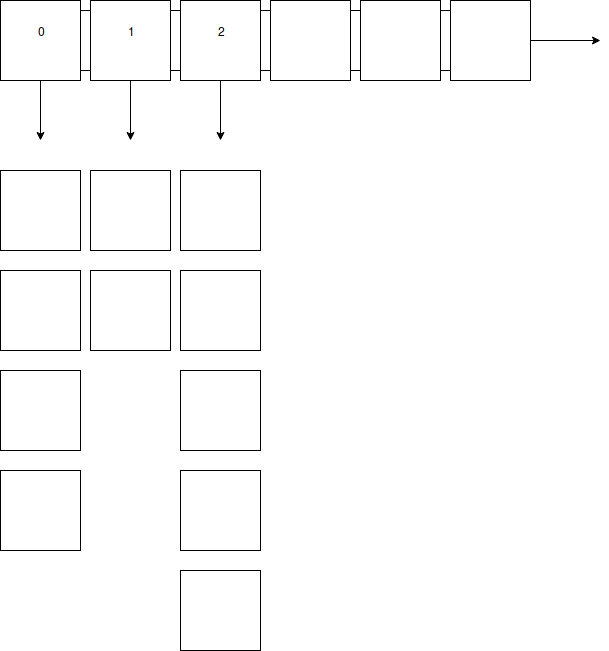
\includegraphics[width=0.7\linewidth]{message_storage}
    \caption{A graphical representation of the BlckchnMsgStorage internal array. The array contains three initialized contacts with a variable number of messages each.}
    \label{fig:messagestorage}
\end{figure}

\subsubsection{Identity Management}
\gls{Identity management} relies on a second \gls{smart contract}\index{smart contract} capable of attaching a single unique user id (\texttt{addr}) with a single username/email/password set, thereby preventing messages from being sent to the wrong person, similar to a phone number. The \texttt{BlckchnMsgStorage} contract itself only deals with the user's address\index{address}, and without some kind of user management and address\index{address} assignment to act as a key any person would be able to tie in to any address\index{address} and download every message in that address\index{address}'s associated ``mailbox''. The \gls{Identity management}\index{Identity management} smart contract contains a key-value lookup table where every new login is assigned an address\index{address} which is immutably tied to that username. When adding a contact, the only value supplied will be a username, which the identity management contract will use to retrieve an address\index{address} which is never exposed to the end user.

\subsection{Functionality Goals}
\subsubsection{Key Management}
Key management is usually handled through well-known servers set up specifically for distributing public keys. Because the keys used with this system are not OpenPGP-standardized, this method may not work as cleanly. Further work will be done to determine the remote key management system that makes the most sense for this platform. Internally to a client application, keys are read from files and are then stored in memory as binary public key\index{public key} objects. Each implementation will require its own language's approach to this, for example the Android app will use net.java.Security.PublicKey\index{PublicKey} and the Python implementation (CLI\index{CLI}) will use rsa.PublicKey\index{PublicKey}, both from their language's standard library. Keys, in the initial release of the application, must be exported (either by manually copying the keyfile from the keys directory or by using the eventual Export functionality)\footnote{At the time of writing, the ``Import'' and ``Export'' functionality groups are not yet implemented. When every basic feature of the applications is in place and working, abstraction functions like these will be added.} and sent (by email or similar medium) to the intended contact, who will then move it into their own keys directory (either manually or by using the eventual Import functionality) to be imported when the new Contact object is created.

\section{Component Architectural Design}

\subsection{Blockchain Communication}
The Blockchain module is used to send and retrieve message packets serialized as strings.

\subsubsection{def get\_identity(self, uname: str) $\rightarrow$ int}
Either produces a new address by which a new user can be contacted or retrieves an existing user's unique address.
\subsubsection{def get\_my\_identity(self, uname: str, password: str) $\rightarrow$ int}
\subsubsection{def new\_identity(self, uname: str, password: str) $\rightarrow$ int}
\subsubsection{def get\_balance(self) $\rightarrow$ float}
Returns the volume of \gls{Ether}\index{Ether} (ETH) the user has in their account. This is used to ensure that a user can always keep track of their ETH\index{ETH} and to keep from running out of currency to cover the gas fees associated with sending messages.
\subsubsection{def submit(self, message: Message)}
Produces a message packet from a database Message object and transmits it to the \gls{blockchain}\index{blockchain}.
\subsubsection{def retrieve(user: Contact, last\_message: int, contact\_list: List[Contact]) $\rightarrow$ List[Message]}
Requests every message packet with an ID later than \texttt{last\_message}, receives a string containing each message packet, and processes the string to pass of for cryptographical processing.

\subsection{Low-Level Cryptography}
This module will provide an abstraction level to an internal language-level implementation of RSA\index{RSA} public/private key encryption\index{encryption}.

\subsubsection{def generate\_key(uname: str)}
Used when logging in for the first time on a new device. Produces a new RSA\index{RSA} keypair.
\subsubsection{def import\_key(uname: str)}
Brings an existing RSA\index{RSA} keypair into memory for application use.
\subsubsection{def encrypt(to: Contact, msg: str) $\rightarrow$ str}
Encrypts a given string \texttt{msg} for decryption by \texttt{to}.
\subsubsection{def decrypt(msg: str) $\rightarrow$ str}
Decrypts messages encrypted with the currently signed-in user's encryption\index{encryption} key.
\subsubsection{def sign(msg: Message) $\rightarrow$ str}
Produces a text-encoded signature\index{signature} for the given message which can then be used to verify the identity of the sender.
\subsubsection{def verify(from: Contact, msg: Message) $\rightarrow$ bool}
Verifies that a message originates with the sender it claims to be from.

\subsection{Database Design}
The database specification is to provide a language-native ``list'' implementation of each necessary object for comparably efficient and low-level data storage and retrieval. These will be frozen in place and saved to files (by way of libraries and utilities like Python's \texttt{shelve}) that will be read and written in chunks which will remove the need for large, complex database files with a more prohibitive overhead. The specific data structures and their interactions are outlined in the \textbf{Data Structure Overview}. Each operation that updates the state of the in-memory database (insert/delete) will cause the database to update on disk as well.

\subsubsection{def insert(msg: Message) $\rightarrow$ bool}
Creates a new database entry with the given Message object.
\subsubsection{def read(id: int) $\rightarrow$ Message}
Returns the message with the given unique identifier.
\subsubsection{def delete(id: int) $\rightarrow$ bool}
Removes the message with the given unique identifier. DOES NOT modify the message records on the \gls{blockchain}\index{blockchain}.
\subsubsection{def new\_contact(addr: int, uname: str, email: str) $\rightarrow$ bool}
Produces a new contact from the given information and adds it to the in-memory database.
\subsubsection{def read\_contact(self, uname: str) $\rightarrow$ Contact}
\subsubsection{def del\_contact(addr: int) $\rightarrow$ bool}
Removes a given contact (identified by \texttt{addr} from the database.)

\section{Real-Time Design}
Real-time interactions are limited by the responsivity and reactivity of \gls{Ethereum}\index{Ethereum}. For multiple users sharing a local node\index{node}, the transmission of messages across blockchains\_message is instantaneous. For a number of node\index{node}s connecting together the transmission of messages is limited by a myriad of factors including the user's network speed and the number of transactions\index{transactions} being processed by \gls{Ethereum}\index{Ethereum} as a whole. When a message is sent, a new transaction\index{transaction} is appended to the \gls{blockchain}\index{blockchain} containing the information relevant to the message being sent. This must propagate through \gls{Ethereum}\index{Ethereum} before it can be loaded into blockchain\_message by the intended recipient, which introduces a delay which is noticeable but not strictly prohibitive.

\section{User Interface Design}
Any implementation of the system should provide a clear, usser-friendly manner of exposing every function of the library to the user. It should also focus heavily on abstracting complex tasks such as key management\index{key management} from the user and presenting such intensive actions in as clear and simple a manner as possible. For the purposes of this project, two implementations are currently under development, the command-line interface that encompasses the end goal of the UI component of the project, and an Android application that will explore the practicality of using a mobile device for such a task.

\subsection{Command-Line Interface}
The CLI\index{CLI} implementation provides all of the basic functions of the system in a bare-bones, low abstraction manner. Each high-level operation provided by the blockchain\_message system should have a 1:1 relationship with a single command (e.g. write message, download messages, read messages, list contacts, et cetera).

\subsection{Graphical/Mobile}
Graphical implementations of blockchain\_message, including the Android application being developed for this project, should provide a highly user-friendly and abstracted way of interacting with the underlying platform.

\section{Help System Design}

\subsection{CLI\index{CLI}}
The CLI\index{CLI} version will include a standard \verb|help| directive that will print out the full list of commands available with usage details for every component in the style of classical *nix command help dialogues. The user manual will also contain specific information on the usage of the CLI version, since that will most directly reflect the functionality described in the original proposal.

\subsection{Graphical/Mobile}
The graphical implementations (starting with the Android app) will contain a help dialog, clearly labeled as part of an auxiliary menu, that will display a clear overview of how every component of the UI will function as well as basic overviews of cryptographical functions and how to interact with an individual \gls{Ethereum}\index{Ethereum} account.

\section{Data Structure Overview}
\subsection{Contact}
Every person that the user interacts with will be stored as a Contact object such that the system can easily exchange messages while maintaining a high level of convenience for the end user.

\subsubsection{addr}
A numerical identifier providing the system with a simple way of addressing and indexing messages.

\subsubsection{uname}
The contact's chosen username, which will be used internally to connect an \texttt{addr} with a more intuitive name and ensure that each address\index{address} is only used once per blockchain\_message environment.

\subsubsection{emailAddress}
The user's given email address\index{address}, which will be used to identify public encryption\index{encryption} keys.

\subsubsection{publicKey}
The public key\index{public key} associated with the given email address\index{address}, stored as Java's internal PublicKey\index{PublicKey} class, Python's rsa.PublicKey\index{PublicKey} class, or a similar data structure.

\subsection{Message}
This data object will be 

\subsubsection{id}
A unique identifier supplied to each message.

\subsubsection{to}
The unique user address\index{address} for the person receiving the message.

\subsubsection{from}
The unique user address\index{address} for the person sending the message.

\subsubsection{text}
Used to store the plaintext \textit{and} ciphertext representations of the message being sent.

\subsubsection{sign}
Contains a text-encoded representation of the RSA\index{RSA} signature\index{signature} applied to the plaintext message.

\subsubsection{verified}
A Boolean value used in client implementations to easily store whether or not the message has been cryptographically verified. When sending to \gls{Ethereum}\index{Ethereum} this will default to false.

\chapter{System Testing Specification}
\section{Testing Overview}
The Python language environment provides several well-constructed frameworks for testing automation. The framework used in this project is \texttt{unittest}\cite{unittest}\index{unittest}, which allows for the creation of structured unit-, class-, and module-level tests. Each level of the application is tested through a dedicated testing module containing logic designed to verify expected behavior on every function and every interconnected set of functionalities. The final product will be considered acceptable for a shipment-ready release when it can be verified that a user can log in, transmit a message\index{message} to another user, and retrieve a message\index{message} sent to them.

\section{Blockchain}
Blockchain interaction tests require that a test \gls{node}\index{node} be running during testing with the two blockchain\_message \glspl{smart contract}\index{smart contracts} deployed. These will make a series of transactions\index{transactions} to \gls{Ethereum}\index{Ethereum}, but will not be concerned with testing the behavior of the \glspl{smart contract}\index{smart contracts} themselves, they will only be concerned with verifying that the client library itself handles the results of the transactions\index{transactions} correctly.
\subsection{Submit}
Ensures that a plaintext message\index{message} sent to \gls{Ethereum}\index{Ethereum} will be accepted without any EVM\index{EVM} errors.
\subsection{Retrieve}
Ensures that a plaintext message\index{message} sent to \gls{Ethereum}\index{Ethereum} can be acceptably retrieved without any EVM\index{EVM} errors or any corruption of data between the application client and the \gls{Ethereum}\index{Ethereum} client.
\subsection{Multiple Retrieve}
If multiple messages are sent to the same person in a row, this test is used to make sure that they will make it to the recipient without corruption and in the correct order.
\subsection{Retrieve User Address}
Given a username, this should create a new user object and ensure that the \texttt{get\_identity} function on the IdentityManager contract returns the correct address corresponding to that user.
\subsection{Create New User}
Given a username and password, these tests should validate that the local authentication system is working properly and that the IdentityManager contract is correctly creating identity entries in the lookup table.

\section{Crypt}
Since the Crypt module is essentially just a thin wrapper to simplify RSA\index{RSA}, these tests will essentially just verify that the \texttt{rsa} library is being used correctly.
\subsection{Encrypt}
Using a contact\index{contact} object with a correct key, we must verify that a given plaintext payload encrypts without throwing any errors.
\subsection{Decrypt}
This test must first encrypt the data for a given \gls{private key}\index{private key}, then verify that it decrypts correctly for that \gls{private key}\index{private key}.
\subsection{Sign}
Using a contact\index{contact} object with a correct key, we must verify that a given plaintext payload can be signed without throwing any errors.
\subsection{Verify}
If a signature cannot be verified, RSA will throw an exception. It must be verified that a correct signature will not throw an exception. This must call the \texttt{sign} function before calling the \texttt{verify} function on the result.

\section{Database}
The database is one of the simplest parts of the program, and as a result these tests will only be required as an automated verification that no breaking changes were made.
\subsection{Insert}
Used to ensure that nothing goes catastrophically wrong when inserting a message\index{message} into the database\index{database}, and that it makes it there as expected.
\subsection{Read}
Proves that the database\index{database} will retrieve the correct message\index{message} when given a message\index{message} address.
\subsection{Delete}
Creates and removes a new message\index{message} entry to ensure that this functionality is in place.
\subsection{Insert Contact}
This ensures that a contact\index{contact} can be added correctly, and that an existing contact\index{contact} won't be added redundantly.
\subsection{Read Contact}
Verifies that the contact\index{contact} retrieved is always the one that is expected.
\subsection{Delete Contact}
Tests that deleting an existing contact\index{contact} will work and that deleting a nonexistent contact\index{contact} will throw an exception correctly.

\section{Integration}
This module will contain one test which connects the functions of the library together in such a way as they will be called in the working application and verifies that none of them cause any catastrophic failures while interacting with one another. We should, at this point, basically be testing that the functions will all continue behaving as expected when 'glued' together.

\section{Interactive CLI Testing}
Since successful automated tests cannot be the only factor that is used to judge a system ``ready'', the bulk of testing will be carried out by simply using the application as intended. Messages will be exchanged over an \gls{Ethereum}\index{Ethereum} test node, approximately imitating the behavior of the \gls{smart contract}\index{smart contract} when running ``in the wild''. A set of test uname/email/password combinations will be used to generate test keys, create contact\index{contact} entries, and exchange messages. This will allow for a thorough overview of application function to note where any issues might be occurring. While the automated tests will be more useful for tracking down the sources of such issues, this will be imperative for ensuring that the entire application functions correctly on a system level.

\section{Smart Contract Testing}
Frameworks for testing \gls{Ethereum}\index{Ethereum} contracts are considerably less mature than for other languages or platforms. Using the Remix IDE\footnote{remix.ethereum.org}, it's possible to develop and debug \glspl{smart contract}\index{smart contracts}, but testing is currently limited to calling individual functions and verifying that they return the expected values. Other solutions exist, but with their own quirks and complications that add to the required software for this project far beyond its original scope. These function calls were addressed by writing comprehensive tests of the Python functions which verified expected responses from the EVM\index{EVM}.

\chapter{User Manual}
\section{Introduction}
blockchain\_message aims to provide a simple, usable way to send encrypted messages in a way that saves them irreversibly without needing to rely on a centralized storage location. The program is developed with security, privacy, and decentralization in mind by using the \gls{Ethereum}\index{Ethereum} world computer. It should serve as a warning, however, that users would be better off if they were somewhat comfortable with \gls{command-line}\index{command-line} programs.

\section{Introductory Manual}
\subsection{General Use}
The interface consists of eight commands for interacting with the message record and the user's contact database.\\

{\raggedright{}
    \texttt{balance} - Check the Ethereum account's balance. This volume of Ether is used to fuel the transfer of messages.\\
    \texttt{check} - See if any new messages have been received.\\
    \texttt{read} - Read all of the messages we've already downloaded.\\
    \texttt{write} - Compose, encrypt, and send a new message. This will prompt for a username to send to, followed by message text. All other steps are handled automatically.\\
    \texttt{contacts} - List the user's current contacts.\\
    \texttt{new-contact} - Create a new contact object. This will prompt for a username and will find the target's address automatically. A public key for the given username must be found in the \texttt{client/.keys/} directory.\\
    \texttt{help} - Display this command list as a help dialog in the context of the running program.\\
    \texttt{exit} - \textit{Always} use this to end the program. It's responsible for ensuring the application's internal state saves correctly.\\
}

\subsection{Help System}
blockchain\_message's ease of use is a very high priority, so as much of the background functionality as possible has been abstracted down to the 8 commands. The help system is split into a command directory that can be called up by typing \texttt{help}, and a set of helpful error messages when any internal errors (trying to send messages to an unknown contact, failed login, et cetera) occur.

\section{System Reference Manual}
\subsection{Service Directory}

\subsubsection{Contact/Identity Management}
On a user's first login, a new entry is created on \gls{Ethereum}\index{Ethereum} that can be used to look up their address number (think of it as being like an email address or phone number) by their username. This makes it so we can add contacts quickly and easily just by knowing their username, and allows logging in without having to remember your own address number every time.
\subsubsection{Encryption Key Management}
Encryption keys are created every time a new user is registered and stored in the \texttt{client/.keys/} directory. These are used to encrypt/decrypt messages and ensure that the sender/recipient is provably the person they say they are.
\subsubsection{Message Send/Receive}
The send/receive process is fairly abstracted so that none of the details need to be handled by the end user. The sender provides a username and message text, and blockchain\_message handles locating the recipient and encrypting the message for their \gls{public key}\index{public key}, then commits the resulting packet to \gls{Ethereum}\index{Ethereum}.

\subsection{Error Recovery}
There may be some issues which the system cannot handle gracefully, such as any errors in communicating with \gls{Ethereum}\index{Ethereum}. If such a crash occurs, first check that your \gls{Ethereum}\index{Ethereum} \gls{node}\index{node} is running correctly, not reporting any errors of its own, fully \gls{synced}\index{synced}, and listening on port 7545. Additionally, ensure that you are running the program through the \texttt{blckchnmsg} script from a terminal emulator\footnote{Terminal on Linux or macOS} or command prompt on Windows\footnote{This can be found by opening the start menu and searching for Command or cmd.} with the current working directory at the root of the program's files. Issues which have been encountered and/or fixed during development are outlined in section 7.1 of this document.

\subsection{Installation}
This installation guide assumes an Ubuntu or Debian Linux derivative, but the installation process can be adapted slightly to fit any Linux distribution. Windows and macOS are supported as well, but with some more work required. blockchain\_message requires that Python\footnote{https://www.python.org/} and the PIP package manager\footnote{https://pypi.org/project/pip/} be installed. The application's \glspl{dependency}\index{dependencies} can be secured by running the \texttt{install} script at the root of the project as root. It will also require an \gls{Ethereum}\index{Ethereum} \gls{node}\index{node} running locally (the program can be modified to allow for using a remote \gls{node}\index{node}), Geth\footnote{https://github.com/ethereum/go-ethereum/wiki/geth} or Parity\footnote{https://www.parity.io/} are both viable options. Once the Ethereum \gls{node}\index{node} is running and \gls{synced}\index{synced} and all of the dependencies installed, the \texttt{blckchnmsg} script will run the program and all first-time setup automatically.\footnote{Users familiar with Python may find it useful to know that blockchain\_message must be installed as a Python package in order to be executed through the client script.}

\pagebreak
\chapter{Appendix}

\section{Known Issues}
\subsection{Message Skip}
If the state of messages on the \gls{blockchain}\index{blockchain} is mismatched with the database, the database may not download further messages or may skip several before continuing to receive.
\subsection{Blockchain out of Message Space}
When the smart contract's internal message space runs out, the client may become unresponsive. \textbf{Addressed by scaling the message space.}
\subsection{Database Corruption}
If the program crashes before data being sent to the database is fully prepared and committed, the database may end up missing data points. This will cause objects to be erroneously set as \texttt{None}, leading to further crashes.

\section{System Evolution}
A number of further improvements for the project have been planned and outlined in this document. The functionality of the system has been laid out in such a way that further implementations can be easily created and tied in with any platform which has a web3 implementation, so my hope is to have more user friendly interfaces (such as an Android application) built for the system. It would also be ideal to improve the cryptography key sharing functions so that users can more easily send public keys to one another.

\addcontentsline{toc}{section}{Listings}
\lstlistoflistings
\begin{adjustwidth}{-50pt}{-50pt}
\lstinputlisting[language=Python,caption={setup.py},label=setup]{setup.py}
\lstinputlisting[language=bash,caption={Installer Script},label=install]{install}
\lstinputlisting[language=bash,caption={blckchnmsg},label=blckchnmsg]{blckchnmsg}
\lstinputlisting[language=C,caption={BlckChnMsgStorage.sol},label=storage]{contract/contracts/BlckChnMsgStorage.sol}
\lstinputlisting[language=C,caption={IdentityManager.sol},label=identity]{contract/contracts/IdentityManager.sol}
\lstinputlisting[language=Python,caption={Contract Deployment Script},label=main]{proof/src/main.py}
\lstinputlisting[language=Python,caption={Contract Deployment Script},label=main]{proof/src/main_test.py}
\lstinputlisting[language=Python,caption={CLI Driver},label=cli]{client/cli.py}
\lstinputlisting[language=Python,caption={Client Module},label=cliinit]{client/__init__.py}
\lstinputlisting[language=Python,caption={Source Module},label=libinit]{blockchain_message/__init__.py}
\lstinputlisting[language=Python,caption={Library Module},label=srcinit]{blockchain_message/src/__init__.py}
\lstinputlisting[language=Python,caption={Main Library File},label=lib]{blockchain_message/src/lib.py}
\lstinputlisting[language=Python,caption={Core Functions},label=core]{blockchain_message/src/core.py}
\lstinputlisting[language=Python,caption={Blockchain Interaction},label=blockchain]{blockchain_message/src/blockchain.py}
\lstinputlisting[language=Python,caption={Cryptographical Functions},label=crypt]{blockchain_message/src/crypt.py}
\lstinputlisting[language=Python,caption={Database Functions},label=db]{blockchain_message/src/database.py}
\lstinputlisting[language=Python,caption={Test Module},label=testinit]{test/__init__.py}
\lstinputlisting[language=Python,caption={Integration Tests},label=testint]{test/test_integration.py}
\lstinputlisting[language=Python,caption={Blockchain Tests},label=testchn]{test/test_blockchain.py}
\lstinputlisting[language=Python,caption={Cryptography Tests},label=testcry]{test/test_crypt.py}
\lstinputlisting[language=Python,caption={Database Tests},label=testdb]{test/test_database.py}
\end{adjustwidth}
\pagebreak
\listoftables
\listoffigures
\printindex\pagebreak
\printglossaries{}
\printbibliography[heading=bibintoc]{}

\end{document}
